\documentclass[10pt,a4paper]{article}
\usepackage[utf8]{inputenc}
\usepackage[T1]{fontenc}
\usepackage[spanish]{babel}
\usepackage{geometry}
\usepackage{graphicx}
\usepackage{booktabs}
\usepackage{float}
\usepackage{array}
\usepackage{xcolor}
\usepackage{url}
\geometry{margin=2.1cm}
\graphicspath{{../../../results/figures/}}
\setlength{\parskip}{0.5em}
\setlength{\parindent}{0pt}
\renewcommand{\arraystretch}{1.12}

\title{Informe final integrado\\EP1 Deep Learning: Fashion-MNIST}
\author{Ignacio Silva \and Lucas Moncada \and Cesar Rojas}
\date{20 de septiembre de 2026}

\begin{document}
\maketitle

\begin{abstract}
Este informe integra el trabajo completo del proyecto: preparación de datos y baseline, estudio de funciones, hiperparámetros y arquitectura, y análisis de optimización, regularización y evaluación final. La configuración se seleccionó exclusivamente mediante validation, se congeló antes de consultar test y obtuvo Accuracy 0,8838 y F1 Macro 0,8836 en la evaluación final única.
\end{abstract}

\section{Objetivo y metodología}

Se entrenó una red neuronal multicapa para clasificar las diez clases de Fashion-MNIST. El diseño experimental fue secuencial y controlado: cada experimento modifica una variable respecto de un control explícito. La selección usa Accuracy, Precision, Recall y F1 en variantes macro y ponderada, curvas de train/validation, gaps de generalización, cantidad de parámetros y costo local cuando corresponde.

El train oficial se dividió de forma estratificada con seed 42 en 54.000 ejemplos de train y 6.000 de validation (5.400/600 por clase). El test oficial de 10.000 ejemplos quedó sellado en E0--E9. Solo después de F0 se hizo una predicción sobre test en F1; sus resultados no habilitaron ningún ajuste posterior.

\section{Datos, preprocesamiento y baseline --- Ignacio}

Fashion-MNIST contiene imágenes de $28\times28$ píxeles en escala de grises. Las imágenes \texttt{uint8} en $[0,255]$ se convierten a \texttt{float32} en $[0,1]$. Las etiquetas se codifican one-hot, coherentes con Softmax y categorical crossentropy. La estratificación conserva la representación de cada clase y hace comparables las métricas de validation.

\begin{figure}[H]
\centering
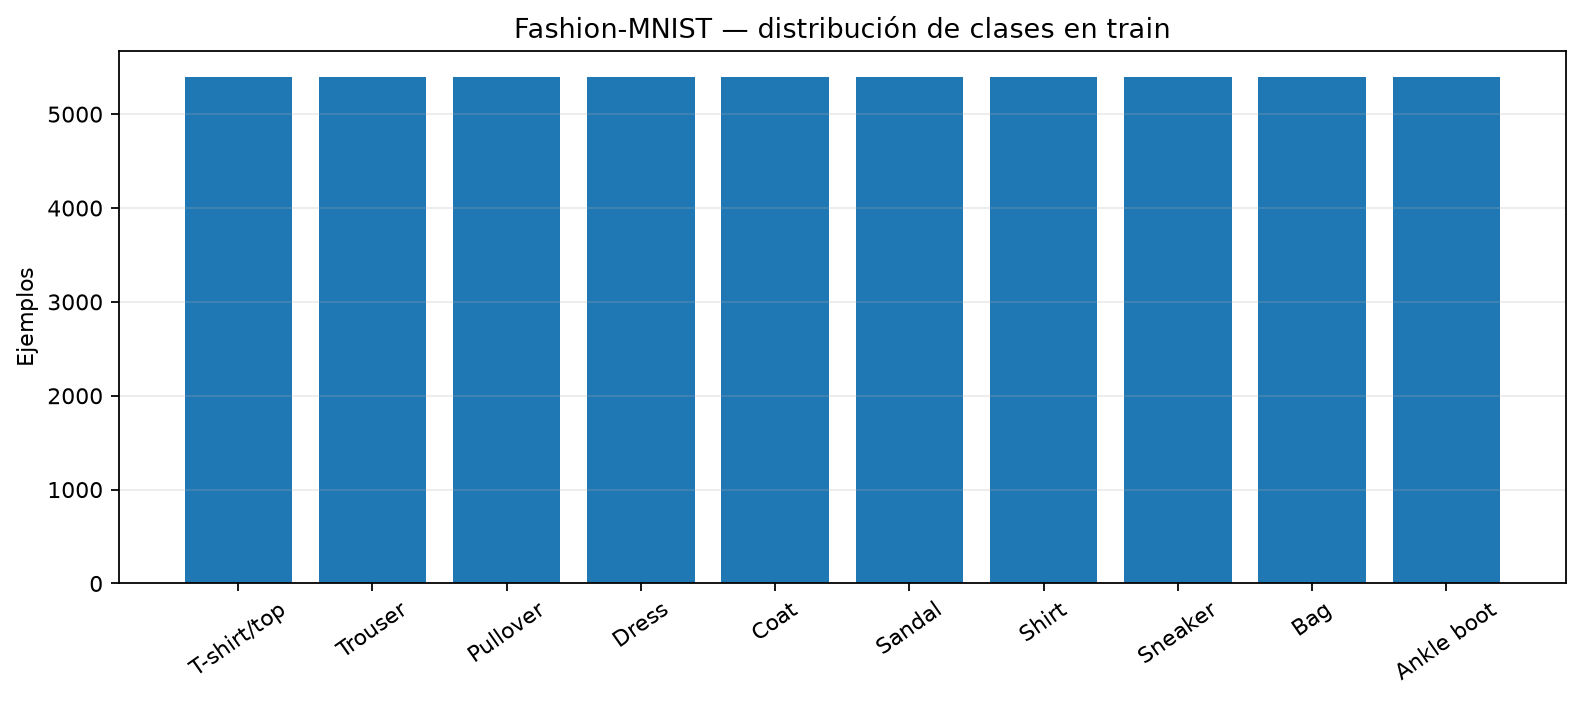
\includegraphics[width=.82\linewidth]{D0_train_class_distribution.png}
\caption{Distribución balanceada de clases en train.}
\end{figure}

E0 usa una MLP con \texttt{Flatten}, capas ocultas $[256,128]$ con ReLU, salida Softmax, categorical crossentropy, SGD con learning rate 0,01, batch 128 y 20 épocas. No usa regularización.

\begin{table}[H]
\centering
\begin{tabular}{lr}
\toprule Métrica de validation & E0 \\
\midrule
Accuracy & 0,8722 \\
Precision Macro & 0,8737 \\
Recall Macro & 0,8722 \\
F1 Macro & 0,8726 \\
Parámetros & 235.146 \\
\bottomrule
\end{tabular}
\caption{Baseline E0 sobre validation.}
\end{table}

\begin{figure}[H]
\centering
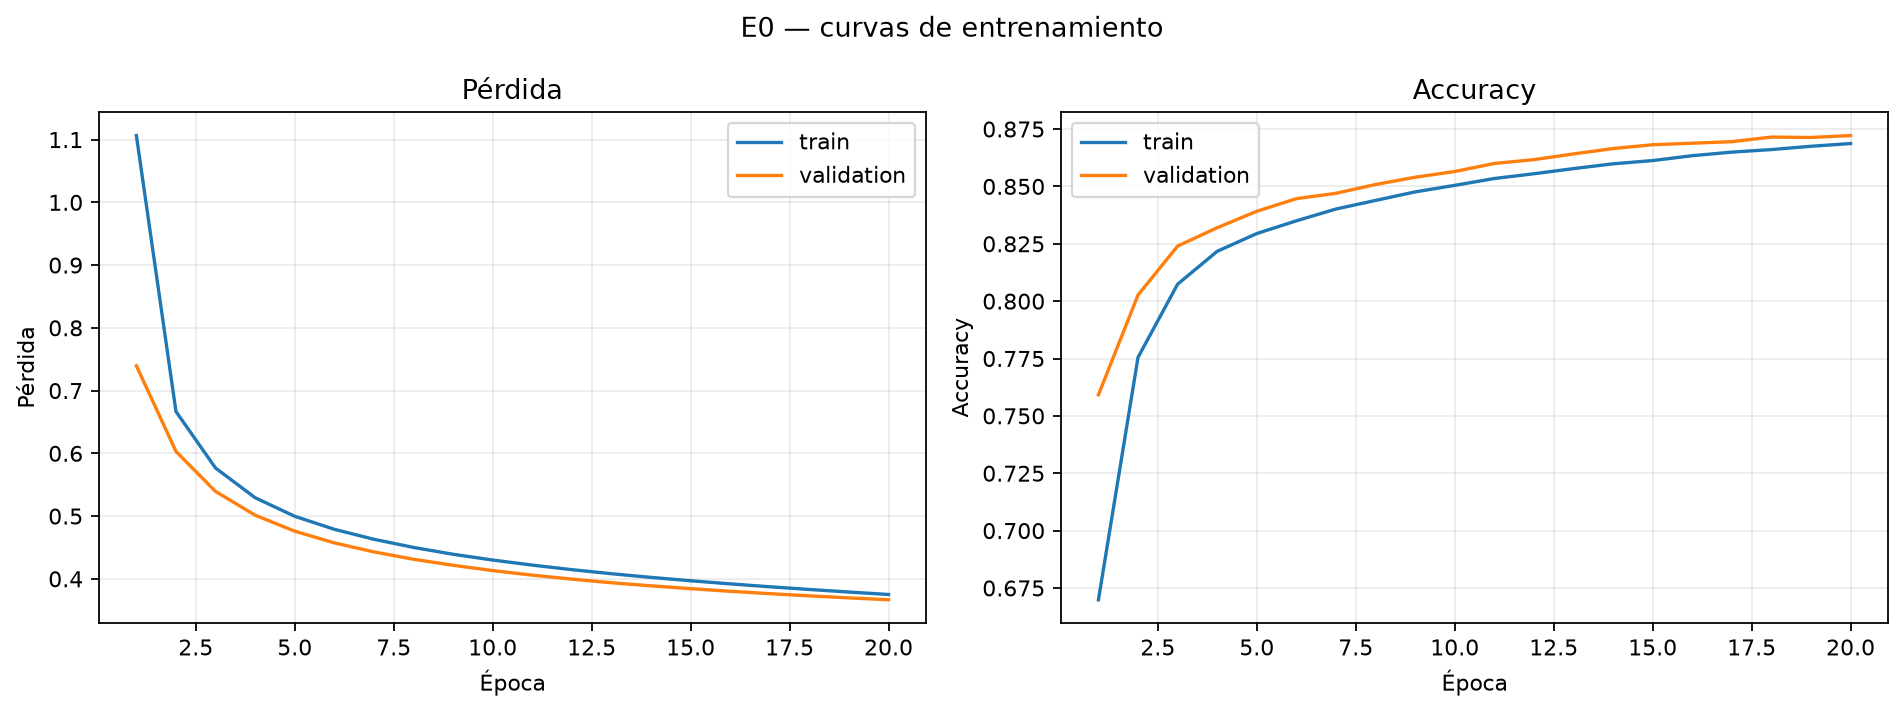
\includegraphics[width=.86\linewidth]{E0_curves.png}
\caption{Curvas de train y validation de E0.}
\end{figure}

\subsection{Activación y función de pérdida}

E1 cambia solamente la activación oculta; E2 cambia solamente la pérdida. ReLU supera a Tanh por 0,78 puntos porcentuales y a Sigmoid por 11,87 puntos de Accuracy. Con ReLU fija, categorical crossentropy supera a MSE por 13,52 puntos. Por ello se conserva ReLU, Softmax y categorical crossentropy para el resto del estudio.

\begin{table}[H]
\centering
\begin{tabular}{llrr}
\toprule ID & Cambio único & Accuracy & F1 Macro \\
\midrule
E0 & ReLU + categorical crossentropy & \textbf{0,8722} & \textbf{0,8726} \\
E1\_tanh & Tanh & 0,8643 & 0,8647 \\
E1\_sigmoid & Sigmoid & 0,7535 & 0,7490 \\
E2\_mse & MSE & 0,7370 & 0,7168 \\
\bottomrule
\end{tabular}
\caption{Comparaciones controladas E1 y E2.}
\end{table}

\begin{figure}[H]
\centering
\begin{minipage}{.48\linewidth}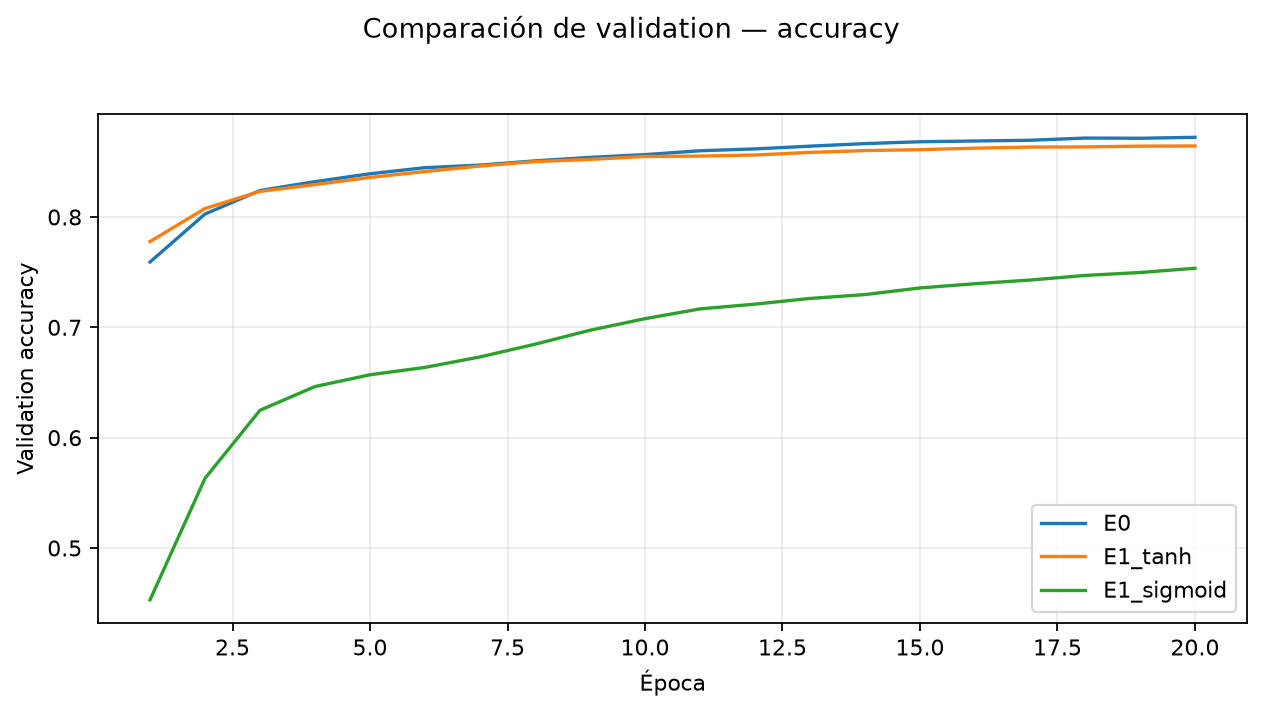
\includegraphics[width=\linewidth]{E1_activation_validation_accuracy.png}\end{minipage}\hfill
\begin{minipage}{.48\linewidth}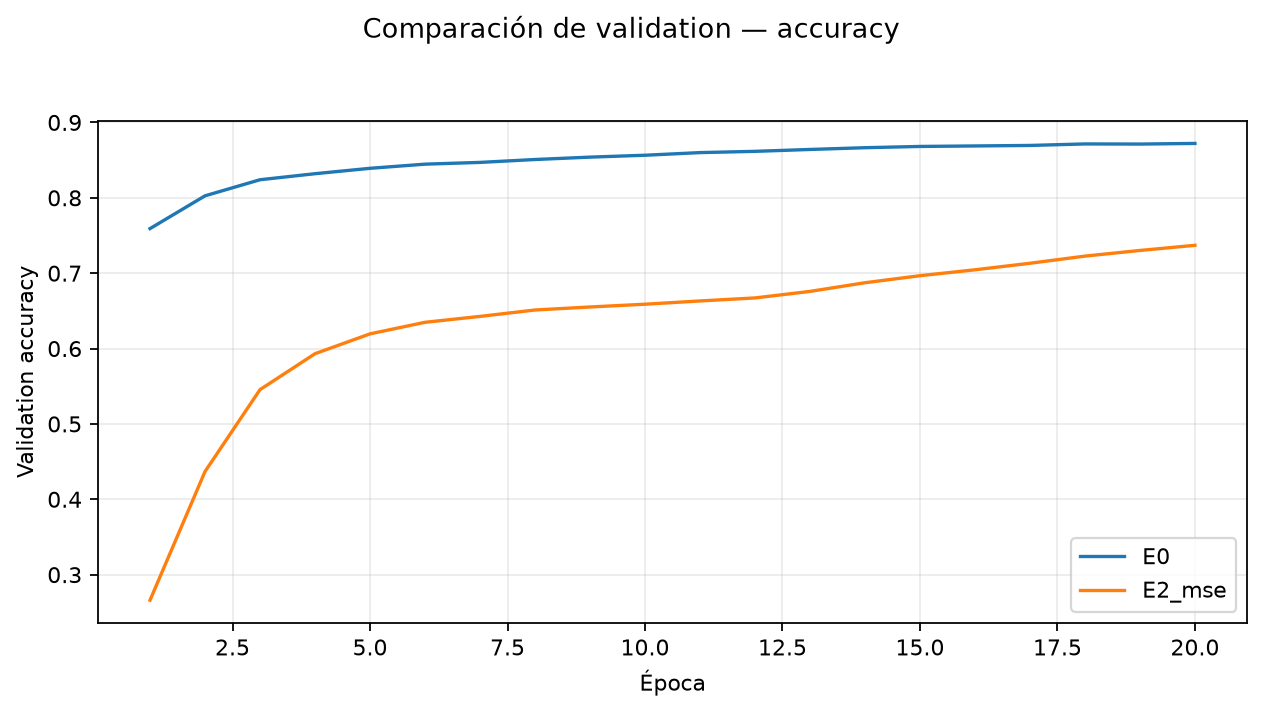
\includegraphics[width=\linewidth]{E2_loss_validation_accuracy.png}\end{minipage}
\caption{Efecto de activación y pérdida sobre Accuracy de validation.}
\end{figure}

\section{Hiperparámetros y capacidad --- Lucas}

E3 compara learning rates 0,001, 0,01 y 0,1. E4 hereda LR 0,1 y compara batch sizes. E5 hereda LR y batch seleccionados y compara capacidad. Esta secuencia evita confundir el efecto de varias variables.

\begin{table}[H]
\centering\small
\begin{tabular}{llrrrr}
\toprule Etapa & Configuración & Accuracy & F1 Macro & Gap loss & Parámetros \\
\midrule
E3 & LR 0,001 & 0,8053 & 0,8034 & --- & 235.146 \\
E3 & LR 0,01 & 0,8722 & 0,8726 & --- & 235.146 \\
E3 & LR 0,1 & \textbf{0,8933} & \textbf{0,8936} & --- & 235.146 \\
E4 & Batch 32 & 0,8860 & 0,8864 & 0,2022 & 235.146 \\
E4 & Batch 128 & \textbf{0,8933} & \textbf{0,8936} & 0,0885 & 235.146 \\
E4 & Batch 512 & 0,8745 & 0,8771 & \textbf{0,0303} & 235.146 \\
E5 & $[64]$ & 0,8873 & 0,8881 & \textbf{0,0256} & 50.890 \\
E5 & $[256,128]$ & 0,8933 & 0,8936 & 0,0885 & 235.146 \\
E5 & $[512,256,128]$ & \textbf{0,8990} & \textbf{0,8989} & 0,1215 & 567.434 \\
\bottomrule
\end{tabular}
\caption{Resultados E3--E5 de validation.}
\end{table}

LR 0,1 mejora 2,12 puntos de Accuracy frente a 0,01. Batch 128 ofrece la mejor métrica con costo intermedio; batch 512 reduce gaps y tiempo, pero pierde 1,88 puntos de Accuracy. La red grande mejora solo 0,57 puntos frente a $[256,128]$, a cambio de 2,41 veces más parámetros y mayor gap. Se selecciona $[256,128]$, SGD, LR 0,1 y batch 128 como control equilibrado.

\begin{figure}[H]
\centering
\begin{minipage}{.48\linewidth}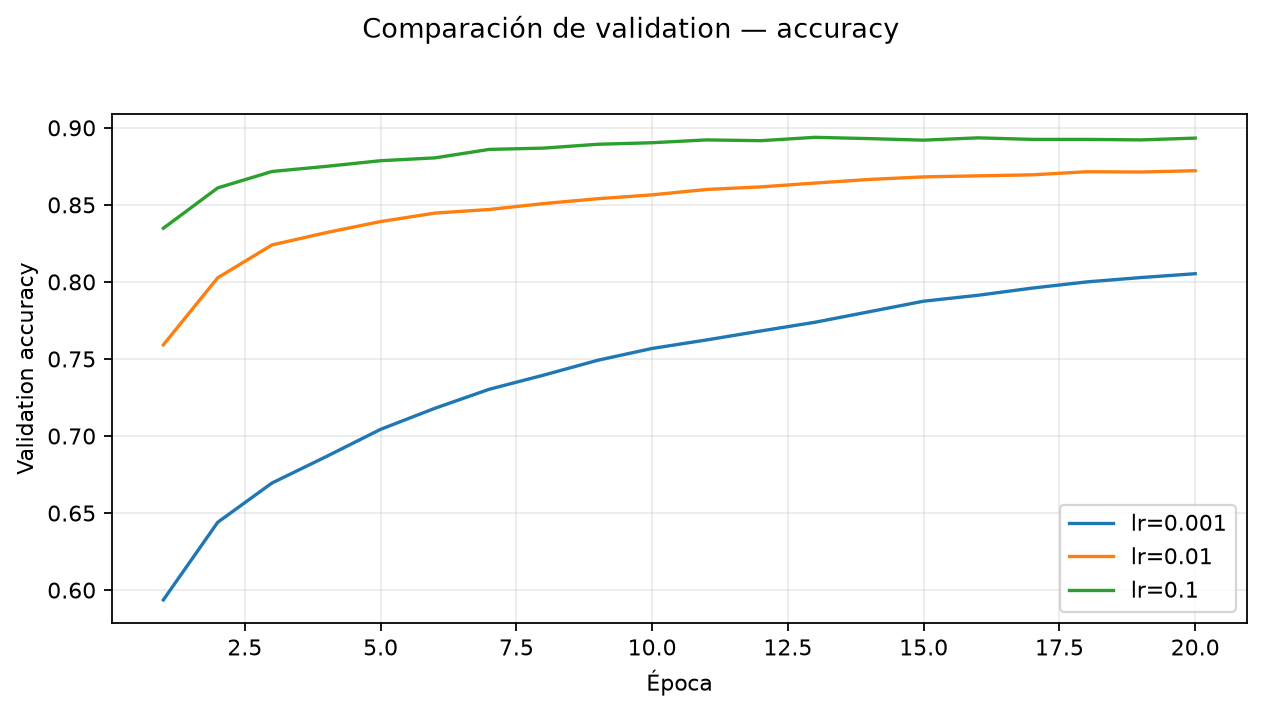
\includegraphics[width=\linewidth]{E3_learning_rate_validation_accuracy.png}\end{minipage}\hfill
\begin{minipage}{.48\linewidth}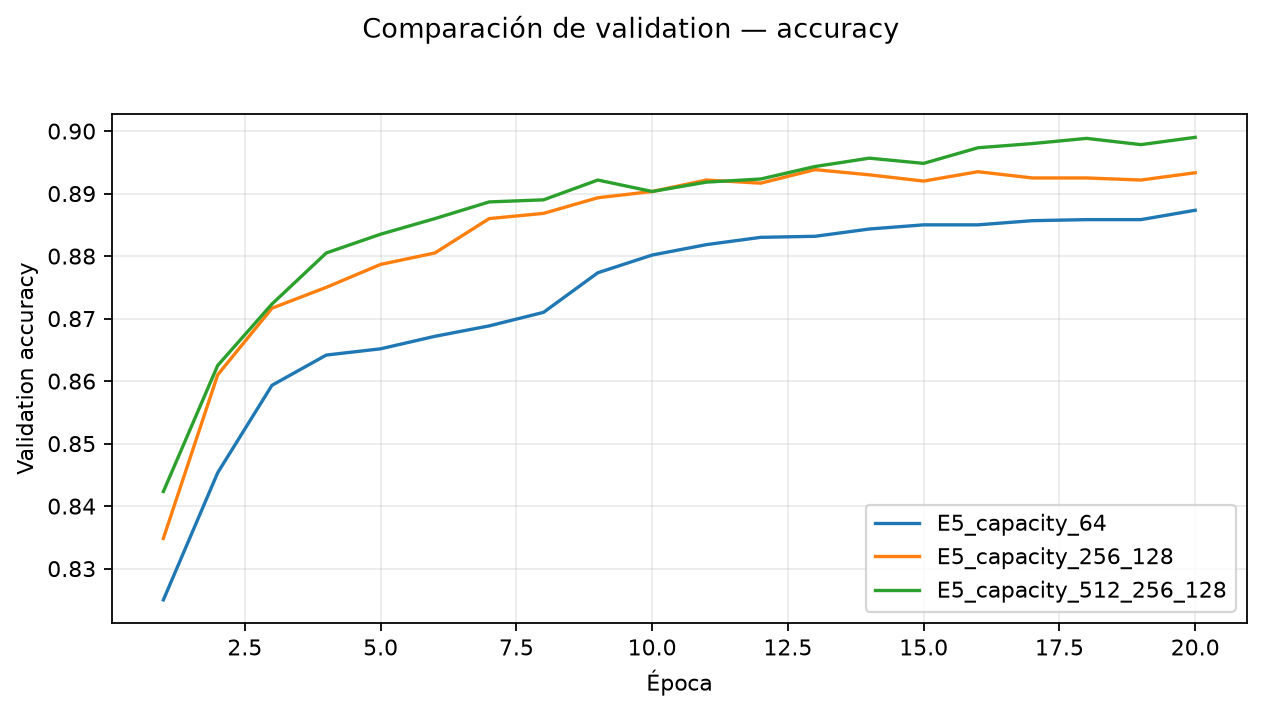
\includegraphics[width=\linewidth]{E5_capacity_validation_accuracy.png}\end{minipage}
\caption{Curvas representativas de E3 y E5.}
\end{figure}

\section{Optimización y regularización --- Cesar}

\subsection{Optimizadores}

E6 sustituye únicamente el optimizador con LR común 0,1. RMSProp y Adam no convergen de manera comparable en esa escala, lo que justifica E6b: con cada optimizador fijo, se cambia solamente el LR a 0,001. SGD mantiene el mejor compromiso, por lo que se usa como control de regularización.

\begin{table}[H]
\centering\small
\begin{tabular}{llrrrr}
\toprule ID & Optimizador / LR & Accuracy & F1 Macro & Gap acc. & Gap loss \\
\midrule
E6 & SGD / 0,1 & \textbf{0,8952} & \textbf{0,8954} & \textbf{0,0287} & \textbf{0,0851} \\
E6 & RMSProp / 0,1 & 0,1985 & 0,0684 & --- & --- \\
E6 & Adam / 0,1 & 0,4722 & 0,4166 & --- & --- \\
E6b & Adam / 0,001 & 0,8912 & 0,8916 & 0,0527 & 0,1941 \\
E6b & RMSProp / 0,001 & 0,8933 & 0,8929 & 0,0476 & 0,2165 \\
\bottomrule
\end{tabular}
\caption{E6 y E6b sobre validation.}
\end{table}

\begin{figure}[H]
\centering
\begin{minipage}{.48\linewidth}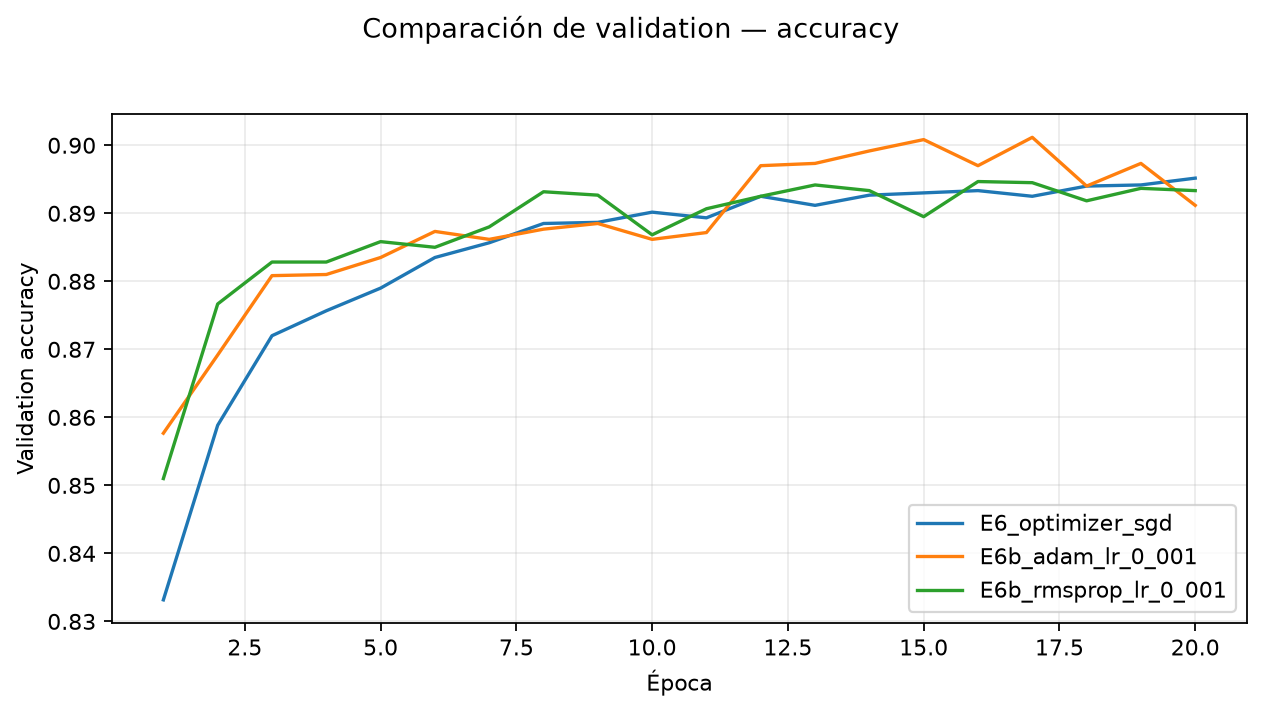
\includegraphics[width=\linewidth]{E6b_retuned_optimizer_validation_accuracy.png}\end{minipage}\hfill
\begin{minipage}{.48\linewidth}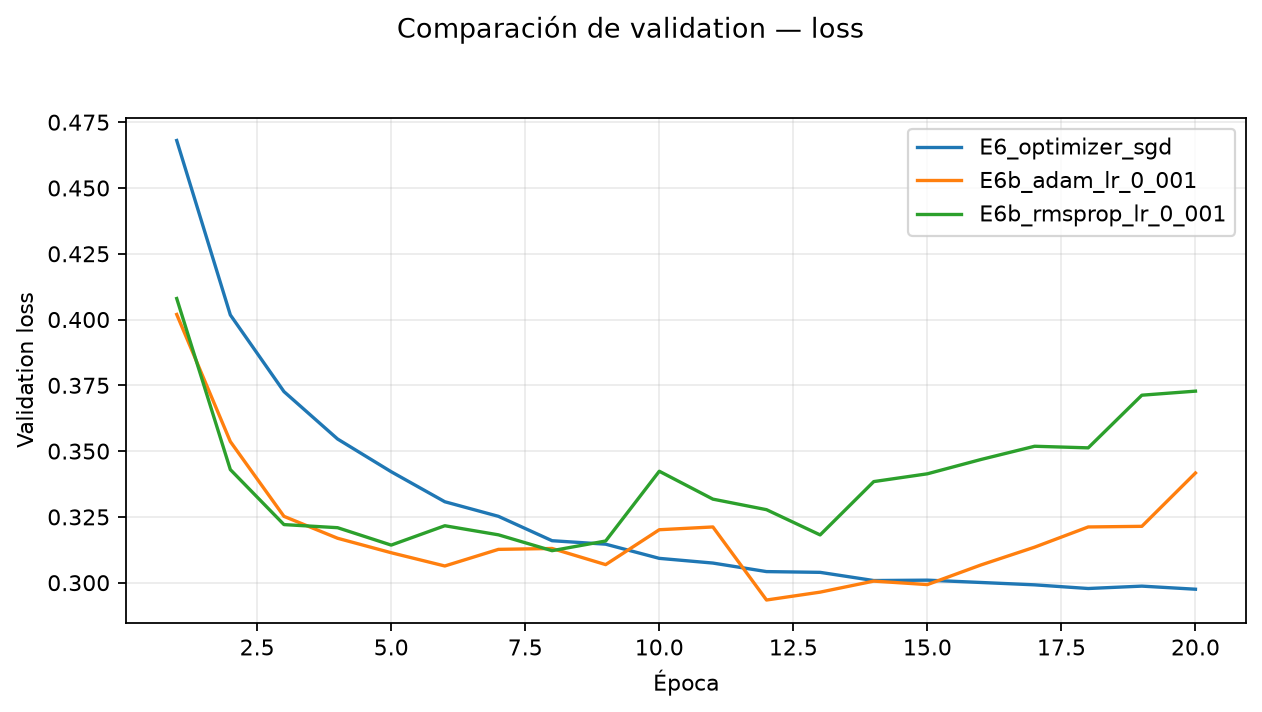
\includegraphics[width=\linewidth]{E6b_retuned_optimizer_validation_loss.png}\end{minipage}
\caption{E6b: LR ajustado de forma separada por optimizador.}
\end{figure}

\subsection{Regularización}

E7 muestra que Dropout 0,2 eleva Accuracy/F1 a 0,8997 y reduce los gaps de Accuracy/loss a 0,0021/0,0135. E8 activa únicamente Batch Normalization en el orden Dense lineal $\rightarrow$ BatchNorm $\rightarrow$ ReLU $\rightarrow$ Dropout; bajo este control, empeora las métricas y gaps. E9 cambia solo L2: $10^{-4}$ baja marginalmente un gap de loss, pero no mejora Accuracy ni F1 y la loss incorpora la penalización.

\begin{table}[H]
\centering\small
\begin{tabular}{llrrrr}
\toprule Etapa & Cambio único & Accuracy & F1 Macro & Gap acc. & Gap loss \\
\midrule
E7 & Dropout 0,0 & 0,8952 & 0,8954 & 0,0287 & 0,0851 \\
E7 & Dropout 0,2 & \textbf{0,8997} & \textbf{0,8997} & \textbf{0,0021} & 0,0135 \\
E8 & BatchNorm OFF & \textbf{0,8997} & \textbf{0,8997} & \textbf{0,0021} & \textbf{0,0135} \\
E8 & BatchNorm ON & 0,8922 & 0,8911 & 0,0294 & 0,0827 \\
E9 & L2 0 & \textbf{0,8997} & \textbf{0,8997} & \textbf{0,0021} & 0,0135 \\
E9 & L2 $10^{-4}$ & 0,8967 & 0,8970 & 0,0025 & \textbf{0,0102} \\
\bottomrule
\end{tabular}
\caption{E7--E9: comparaciones de regularización.}
\end{table}

\begin{figure}[H]
\centering
\begin{minipage}{.48\linewidth}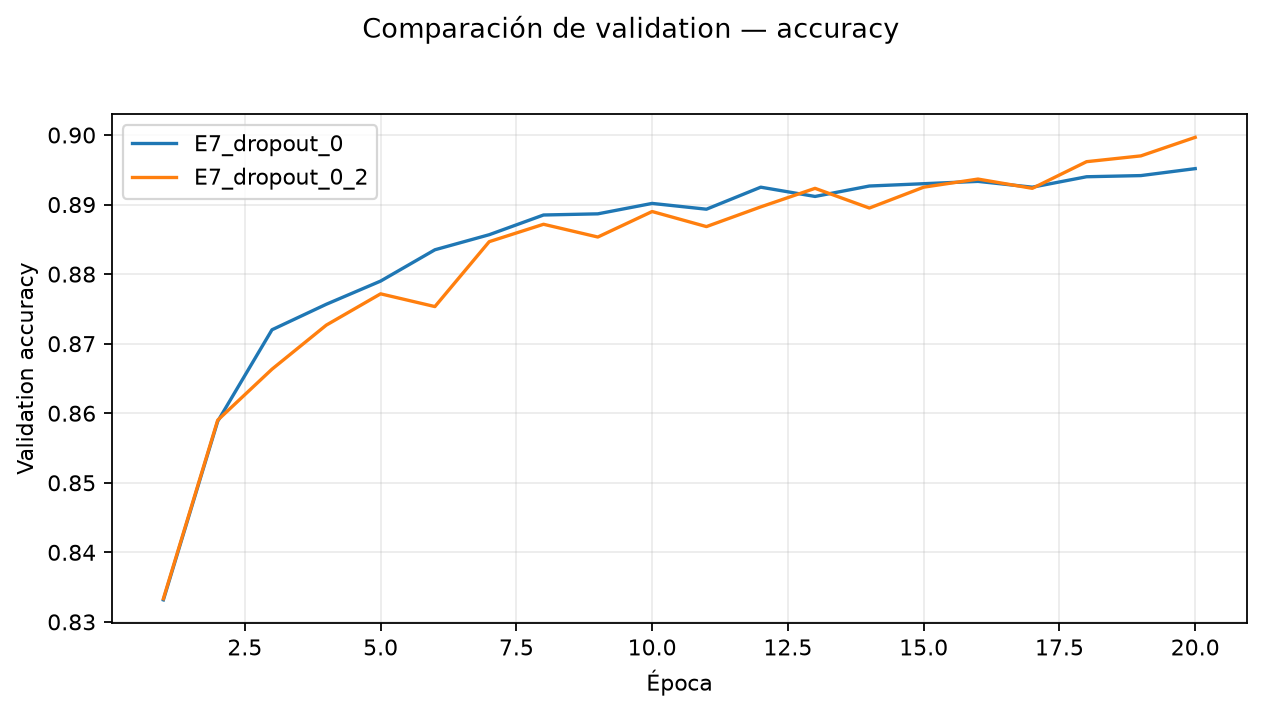
\includegraphics[width=\linewidth]{E7_dropout_validation_accuracy.png}\end{minipage}\hfill
\begin{minipage}{.48\linewidth}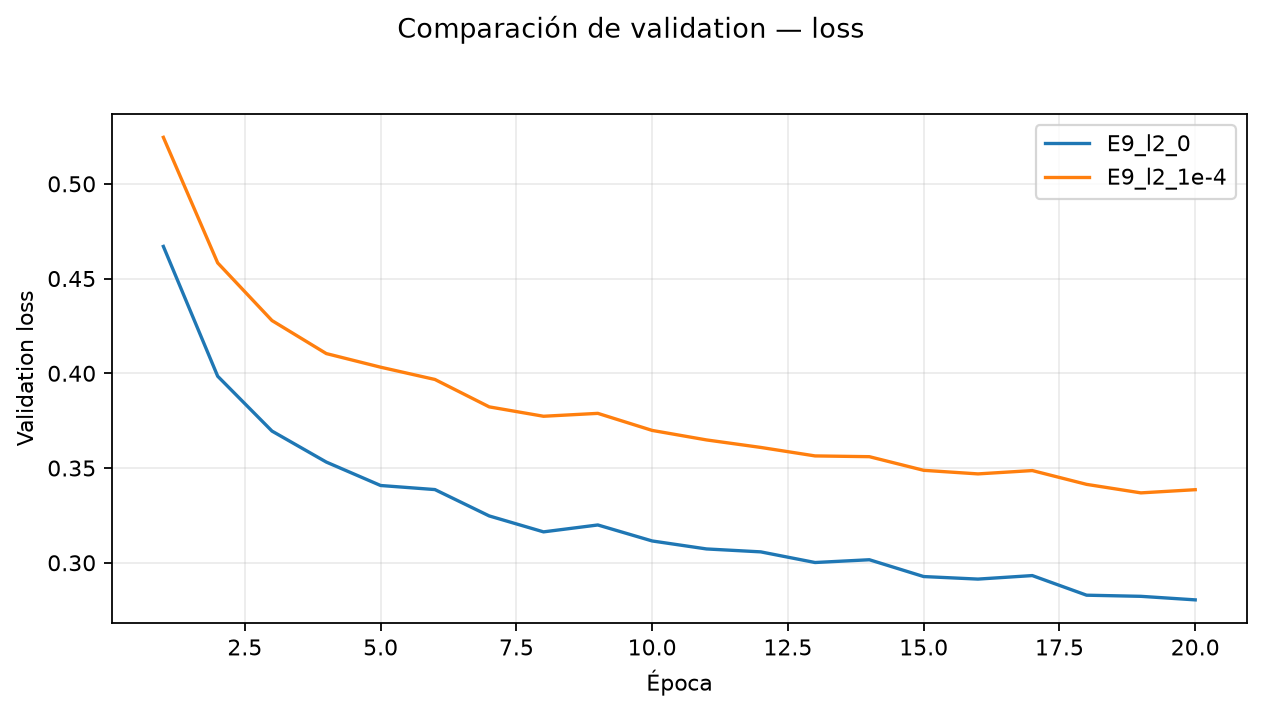
\includegraphics[width=\linewidth]{E9_l2_validation_loss.png}\end{minipage}
\caption{Curvas de validation para Dropout y L2.}
\end{figure}

\section{F0, F1 y análisis final}

La decisión L2 se repitió con seed 7: sin L2 obtuvo Accuracy 0,8902 y con L2 0,8863. Los promedios locales con dos seeds son 0,8949 y 0,8915 respectivamente. Una revisión externa observó una diferencia marginal e inversión en otra ejecución; por ello se mantiene L2 cero como opción prudente y trazable, sin afirmar estabilidad robusta entre entornos. No se activa Early Stopping porque el control alcanza su mejor validation accuracy y loss al final de las 20 épocas, sin deterioro sostenido ni ahorro material.

F0 congela: MLP $[256,128]$, ReLU, Softmax, categorical crossentropy, SGD LR 0,1, batch 128, 20 épocas, seed 42, Dropout 0,2, sin BatchNorm, L2 ni Early Stopping. F1 entrenó esta configuración conservando el split 54.000/6.000 y la evaluó una única vez sobre test. Esa evaluación decisoria queda registrada con el hash de F0 y las versiones del entorno; el notebook de Colab presenta dicho registro y no vuelve a consultar test.

\begin{table}[H]
\centering
\begin{tabular}{lr}
\toprule Métrica & Test \\
\midrule
Accuracy & 0,8838 \\
Precision Macro & 0,8844 \\
Recall Macro & 0,8838 \\
F1 Macro & 0,8836 \\
Precision ponderada & 0,8844 \\
Recall ponderado & 0,8838 \\
F1 ponderado & 0,8836 \\
\bottomrule
\end{tabular}
\caption{F1: evaluación final única sobre los 10.000 ejemplos oficiales de test.}
\end{table}

\begin{table}[H]
\centering\small
\begin{tabular}{lrrr}
\toprule Clase & Precision & Recall & F1 \\
\midrule
T-shirt/top & 0,8721 & 0,7980 & 0,8334 \\
Trouser & 0,9898 & 0,9700 & 0,9798 \\
Pullover & 0,7958 & 0,7990 & 0,7974 \\
Dress & 0,8394 & 0,9250 & 0,8801 \\
Coat & 0,8030 & 0,8070 & 0,8050 \\
Sandal & 0,9795 & 0,9550 & 0,9671 \\
Shirt & 0,7021 & 0,6930 & 0,6975 \\
Sneaker & 0,9238 & 0,9700 & 0,9463 \\
Bag & 0,9710 & 0,9720 & 0,9715 \\
Ankle boot & 0,9674 & 0,9490 & 0,9581 \\
\bottomrule
\end{tabular}
\caption{Métricas por clase en F1. Shirt es la clase más difícil.}
\end{table}

\begin{figure}[H]
\centering
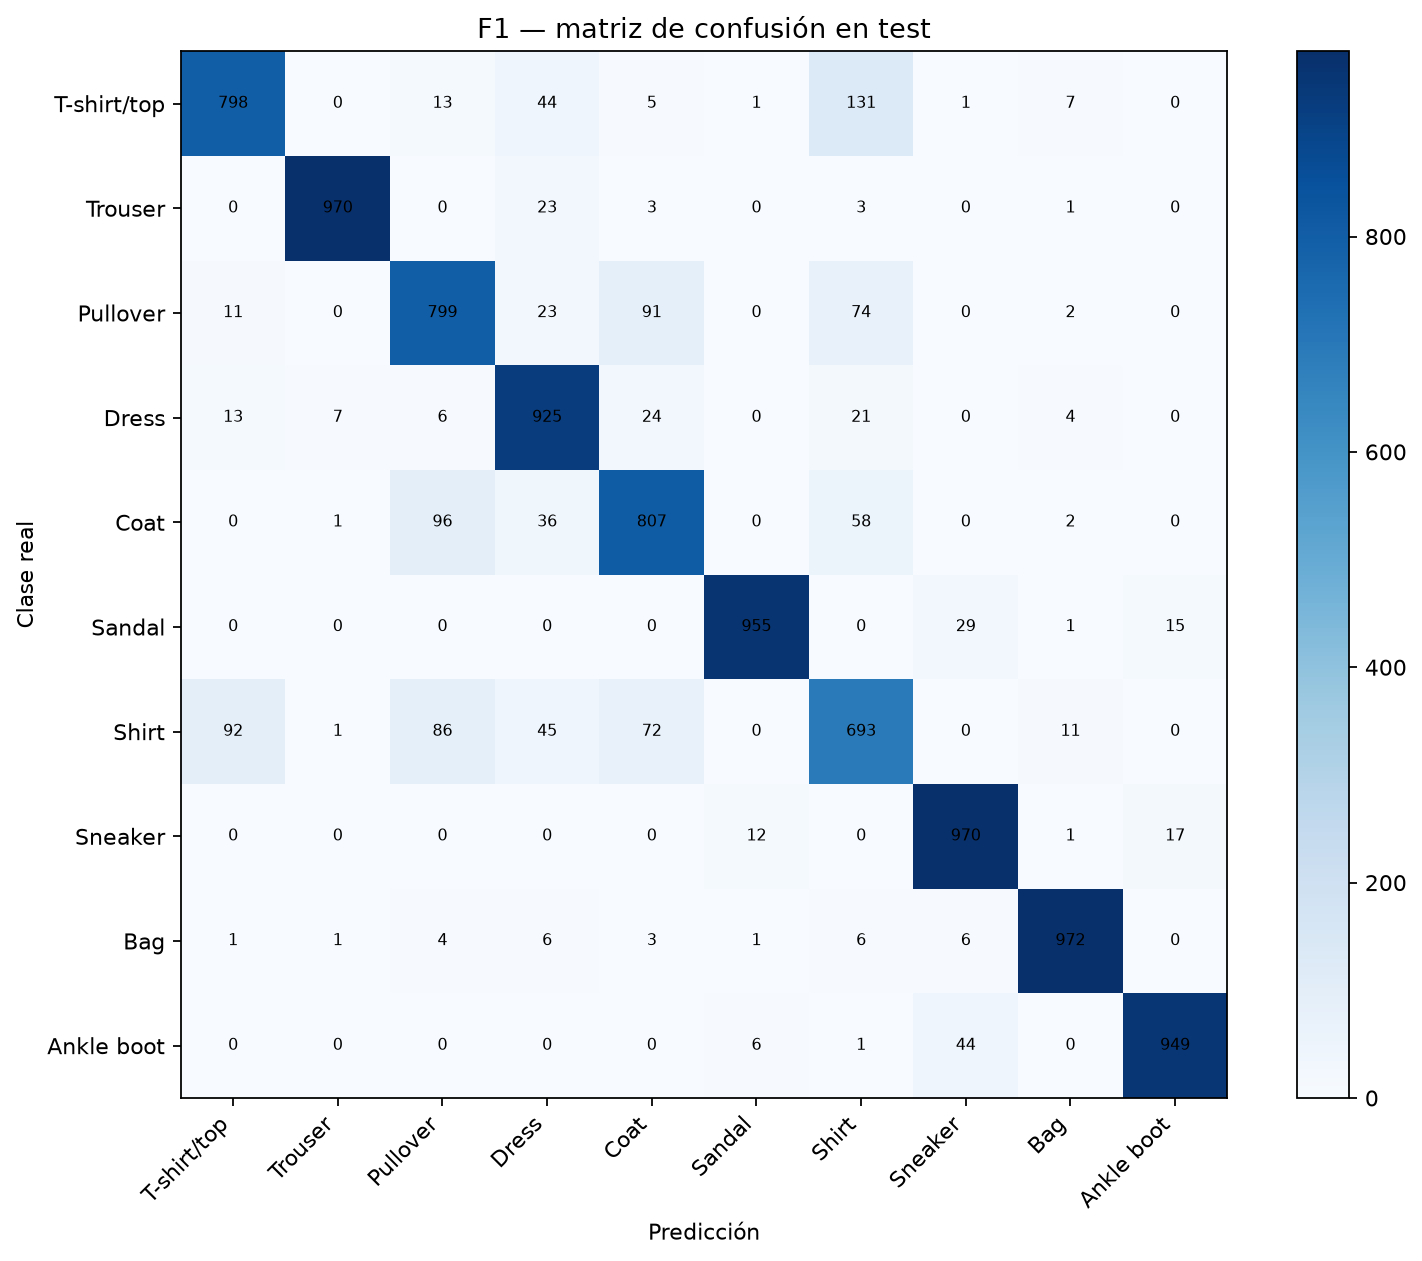
\includegraphics[width=.92\linewidth]{F1_test_confusion_matrix.png}
\caption{Matriz de confusión final. Las confusiones se concentran en prendas superiores visualmente similares.}
\end{figure}

\begin{figure}[H]
\centering
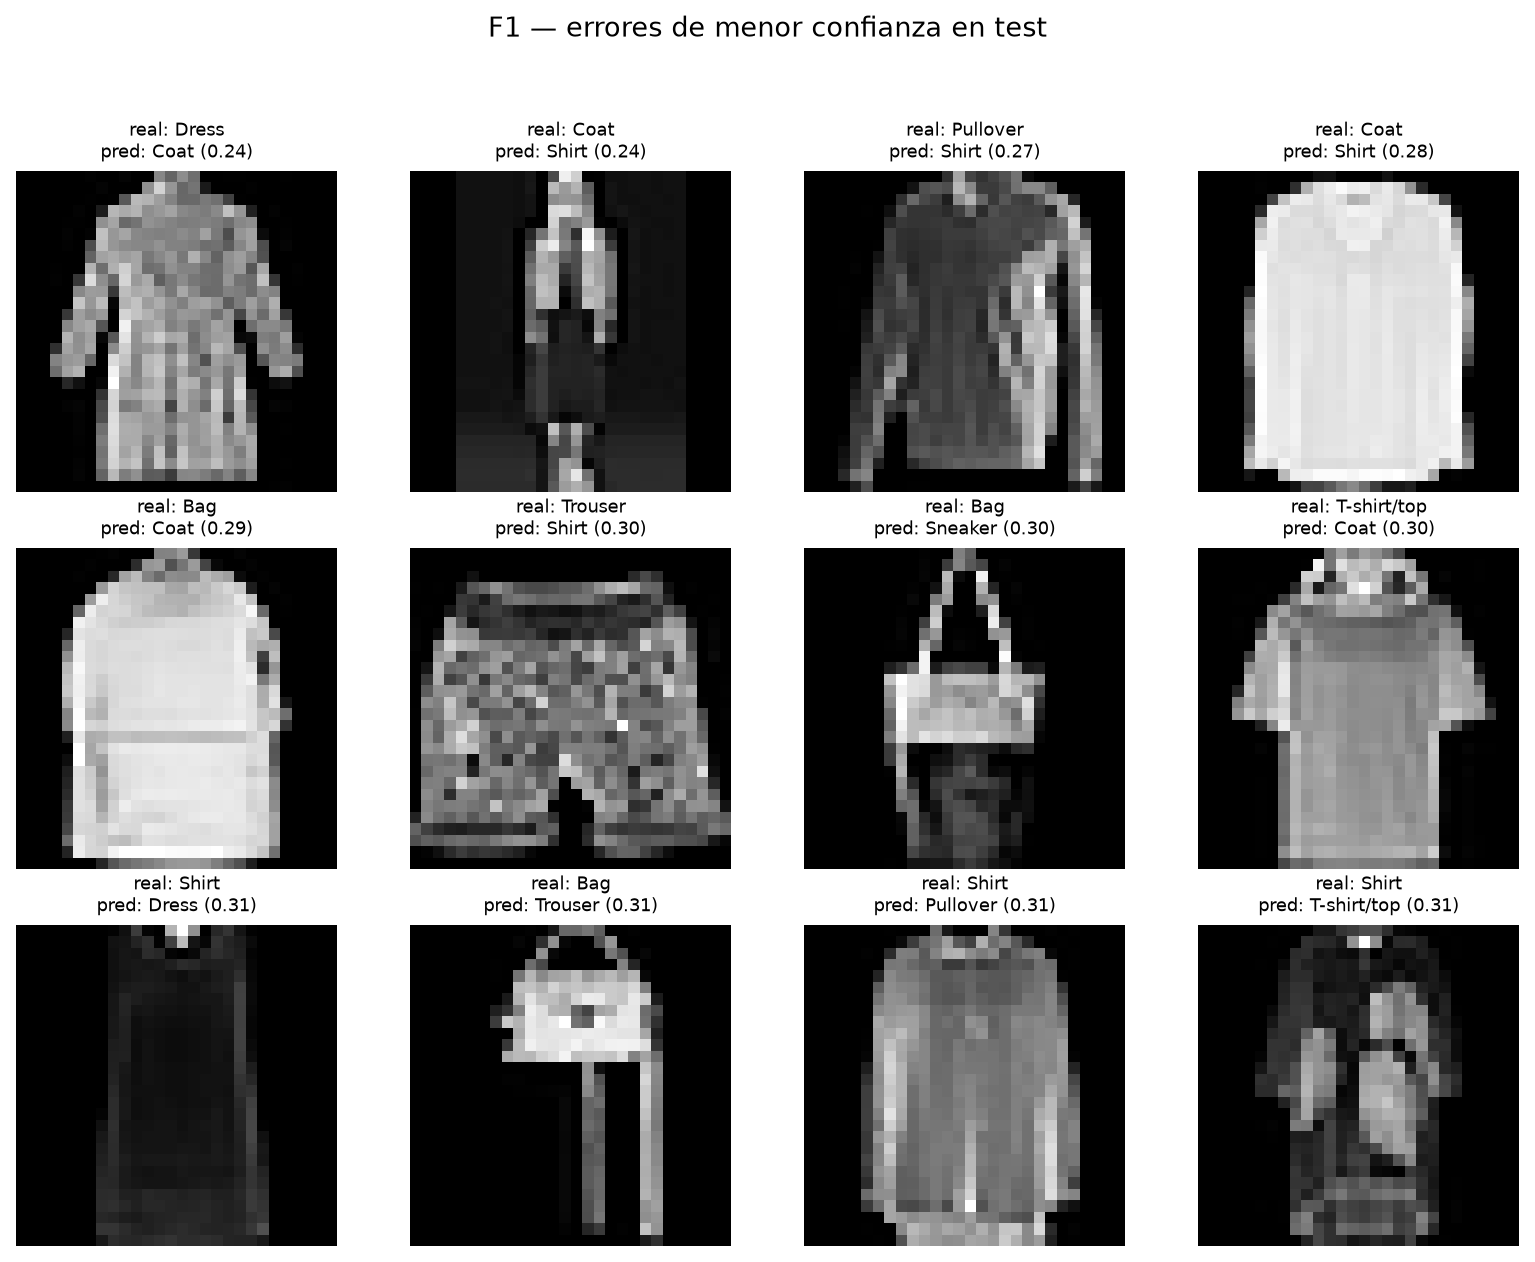
\includegraphics[width=.88\linewidth]{F1_test_low_confidence_errors.png}
\caption{Errores de menor confianza en test; complementan las métricas agregadas.}
\end{figure}

\section{Conclusiones y reproducibilidad}

El estudio respalda una MLP compacta y trazable. ReLU, Softmax y categorical crossentropy fueron las funciones adecuadas; LR 0,1 y batch 128 lograron el mejor equilibrio; la arquitectura $[256,128]$ evitó el incremento desproporcionado de complejidad de la alternativa grande; y Dropout 0,2 fue la mejora de generalización seleccionada. Batch Normalization y L2 no mejoraron bajo estas condiciones, conclusión contextual y no general.

F1 Macro 0,8836 confirma desempeño equilibrado globalmente, pero el análisis por clase revela una limitación importante: Shirt alcanza F1 0,6975 y se confunde con prendas superiores parecidas. Esta evidencia se comunica como limitación; no se usa para modificar el modelo tras test.

La ejecución canónica se identifica con Python 3.12, \texttt{uv sync --frozen} y las versiones bloqueadas en \texttt{uv.lock}. El proyecto cuenta con 31 pruebas automatizadas y lint correcto. El notebook final para Colab clona la rama versionada, presenta código, experimentos, gráficos y conclusiones, y conserva el presupuesto de test al mostrar el registro F1 sin repetirlo.

\end{document}
